%++++++++++++++++++++++++++++++++++++++++
\documentclass[a4paper,11pt]{article}
\usepackage{url}
\usepackage{hyperref}
\usepackage{fullpage}
\usepackage{booktabs}
\usepackage{graphicx}
\usepackage{wrapfig}
\usepackage{caption}
\usepackage{float}
\usepackage{subcaption}
\usepackage{enumerate}
\usepackage{color}
\usepackage{capt-of}
\usepackage{todonotes}
\usepackage{geometry}
 \geometry{
   a4paper,
   total={170mm,257mm},
   left=15mm,
   right=15mm,
   top=15mm,
 }
\usepackage{indentfirst}
  \setlength{\parindent}{0.5em}
  \setlength{\parskip}{0.1em} 
\usepackage{tabularx} % extra features for tabular environment
\usepackage{amsmath}  % improve math presentation
\newcommand{\Test}[1]{\expandafter\hat#1}
\usepackage{graphicx} % takes care of graphic including machinery
\hypersetup{
    colorlinks=true,       % false: boxed links; true: colored links
    linkcolor=blue,        % color of internal links
    citecolor=blue,        % color of links to bibliography
    filecolor=magenta,     % color of file links
    urlcolor=blue
}

% other packages
\usepackage{listings} % code listings
\lstset{framextopmargin=0pt,frame=lines}
\lstset{
    basicstyle=\footnotesize\ttfamily,
    breaklines=true,
    tabsize=4,
    keepspaces=true,
    columns=flexible,
    % backgroundcolor=\color[gray]{0.9},
    frame=single
}

\usepackage{todonotes}

%++++++++++++++++++++++++++++++++++++++++

\begin{document}

\title{
    System Identification \\
    CE-1: Time-domain methods
}
\author{Camilla Carta \\ Michael Spieler}
\date{\today}
\maketitle

\section{Step and impulse response}

In order to analyze the dynamic characteristics of a system, a second order transfer function (see Equation \ref{eq:transfer_func}) was given to be simulated with Matlab environment Simulink. Moreover, it had to follow these parameters:

\begin{itemize}
\item Sample time: $Te = 0.2s$;
\item Measurement noise: $\mu = 0$ and $\sigma^2 = 0.1$;
\item Saturation: $-0.5<INPUT<0.5$.
\end{itemize}

We observe that the sampling period $T_e = 0.2s$ is sufficiently small, given that $\omega_0 = 2s^{-1} \ll \frac{2\pi}{T_e} = 31.4s^{-1}$.

\begin{equation}
	G(s) = \frac{4}{s^2+s+4}
    \label{eq:transfer_func}
\end{equation}

The Simulink model is represented in Figure \ref{fig:simlink}. 

\begin{figure}[H]
	\centering
    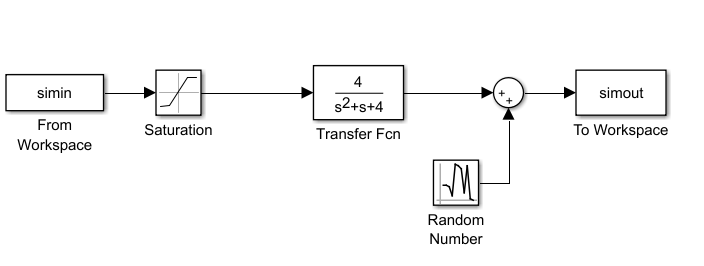
\includegraphics[height=7cm]{images/simlink}
    \caption{Simulink model}
    \label{fig:simlink}
\end{figure}


To begin with, the true step and impulse response were calculated, then compared with the simulated system's responses, which can be seen in Figure \ref{fig:responses_noise}. The step applied in the simulation had a delay of 1s, a length of 50s and an amplitude of 0.5 caused by the Saturation Block; as such, the output was divided by 0.5 in order to estimate the actual response of the simulation. In Figure \ref{fig:step_noise}, the simulated responses (with and without noise) are compared to the real one. 

The same procedure was repeated in order to obtain the impulse response of the system (see Figure \ref{fig:impulse_noise}). As observed before, the input was limited by the Saturation Block, but this time the output was divided by the saturation limit times the sampling time, so as to take into account the difference between a theoretical Kronecker delta and the empirical one, which has a length of Te and an amplitude set by the saturation (also see page 32-33 of the course book).

The images reveal the sensitivity of this method to noise, which covers the response in a significant way, making impossible the characterization of the system. It was noticed that by reducing the noise variance to 0.01, the second order response was considerably clearer and the steady state more stable.



\begin{figure}[H]
\centering
    \begin{subfigure}[t]{0.5\textwidth}
        \centering
        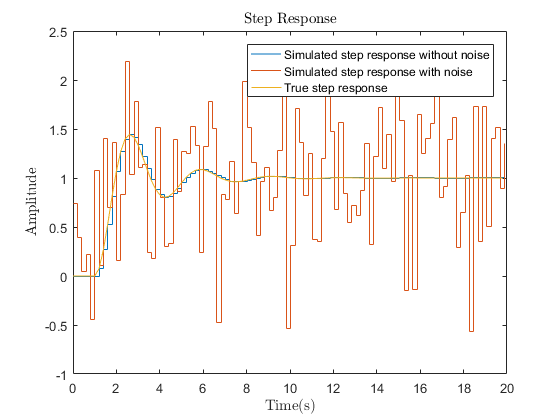
\includegraphics[height=7cm]{images/step_wo_noise} 
        \caption{Real step response against simulated with and without noise}
        \label{fig:step_noise}
    \end{subfigure}
    ~
    \begin{subfigure}[t]{0.5\textwidth}
        \centering
        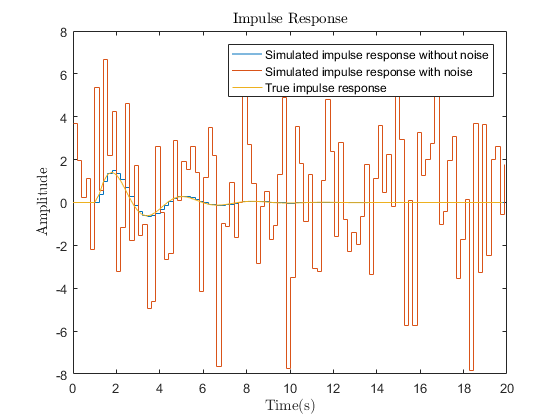
\includegraphics[height=7cm]{images/impulse_wo_noise} 
        \caption{Real impulse response against simulated with and without noise}
		\label{fig:impulse_noise}
    \end{subfigure} 
\caption{Step and impulse response }
\label{fig:responses_noise}
\end{figure}




\section{Autocorrelation of a PRBS signal}

Using the given \textit{prbs.m}, a signal \textit{prbs(n,p)} can be created, with a n-bits register repeated over p periods. Then the function \textit{[R,h] = intcorr(u,y)} was written, which calculates the cross-correlation of same-length signals u and y (see Listing \ref{lst:intcor}). 

The function \textit{intcorr} was tested by calculating the autocorrelation $R_{uu}$ of a signal \textit{u = prbs(5,4)}. The result is given by the Figure \ref{fig:autocorr}, which is coherent with the results shown at page 22 of the course book.

\begin{figure}[H]
	\centering
    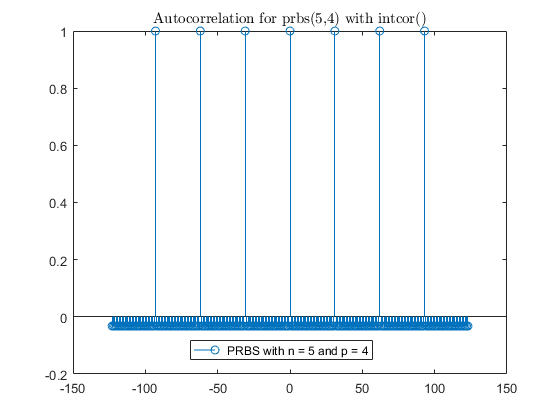
\includegraphics[height=9cm]{images/autocorr_prbs54}
    \caption{Autocorrelation of prbs(5,4) with the function intcorr()}
    \label{fig:autocorr}
\end{figure}



\begin{lstlisting}[language=Matlab,numbers=left,caption=intcor.m,label=lst:intcor]
function [R,h] = intcor(u,y)
% correlation function
% supposes that u and y have same length

N = length(u);
R = [];
h = [];

for h0 = -N+1:N-1
    buff = 0;
    for k = 1:N
        buff = buff + 1/N * u(k)*y(mod(k-h0+N-1,N)+1);
    end
    R = [R;buff];
    h = [h;h0];
end
\end{lstlisting}



\section{Impulse response by deconvolution method}
%\todo[inline]{The code for computing the impulse response by the deconvolution algorithm. The plot of the identified impulse response compared with the true one. Give the 2-norm of the error.}

The impulse response was calculated here by using the deconvolution method, which is presented at the pages 32-34 of the course book. Using an impulse as input and measuring the output, it is possible to calculate the impulse response of a linear system with the Equations \ref{eq:deconv_mat} and \ref{eq:deconv}.

\begin{equation}
\label{eq:deconv_mat}
  \left[ {\begin{array}{c}
   y(0)\\
   y(1)\\
   \vdots \\
   y(N-1)
  \end{array} } \right] 
  = 
  \left[ {\begin{array}{cccc}
   u(0) & 0 & \cdots & 0\\
   u(1) & u(0) & \cdots & 0\\
   \vdots & \vdots & \cdots & \vdots \\
   u(N-1) & u(N-2) & \cdots & u(0)
  \end{array} } \right]
  \left[ {\begin{array}{c}
   g(0)\\
   g(1)\\
   \vdots \\
   g(N-1)
  \end{array} } \right] 
\end{equation}

\begin{equation}
\label{eq:deconv}
\Theta = U^{-1}Y
\end{equation}

As the Toepliz matrix U is ill-conditioned so that $\Theta$ cannot be computed, it is necessary to use the finite impulse response by assuming that $g(k) = 0$ for $k \geq K$, as a stable system's impulse response should converge to zero. 

As such, the Equations \ref{eq:deconv_mat} and \ref{eq:deconv} can be rewritten as   

\begin{equation}
\label{eq:deconv_mat_K}
  \left[ {\begin{array}{c}
   y(0)\\
   y(1)\\
   \vdots \\
   y(N-1)
  \end{array} } \right] 
  = 
  \left[ {\begin{array}{cccc}
   u(0) & 0 & \cdots & 0\\
   u(1) & u(0) & \cdots & 0\\
   \vdots & \vdots & \cdots & \vdots \\
   u(N-1) & u(N-2) & \cdots & u(N-K)
  \end{array} } \right]
  \left[ {\begin{array}{c}
   g(0)\\
   g(1)\\
   \vdots \\
   g(K-1)
  \end{array} } \right] 
\end{equation}

\begin{equation}
\label{eq:deconv_K}
\Theta_K = (U_K^{T}U_K)^{-1}U_K^{T}Y_K
\end{equation}

where $U_K$, $Y_K$ and $\Theta_K$ are truncated versions for a dimensions K to be established. 

In Figure \ref{fig:num_deconv}, the estimated impulse response after truncation with K = 60 can be observed, which corresponds to a simulation of 12s. The 2-norm error was found equal to 2.6326. It can be noticed that the method is sensitive to noise. 

\begin{figure}[H]
	\centering
    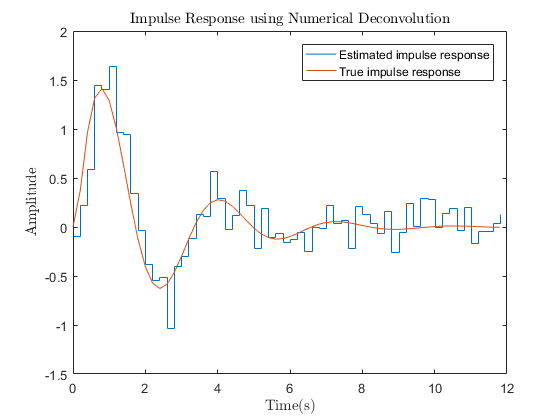
\includegraphics[height=9cm]{images/impulse_num_deconv}
    \caption{Impulse response calculated with the numerical deconvolution method against the real response.}
    \label{fig:num_deconv}
\end{figure}

\begin{lstlisting}[language=Matlab,numbers=left,caption=Numerical deconvolution,label=lst:num_deconv]
Te = 0.2;
sim_time = 70;
N = sim_time/Te;
amplitudeLimit = 0.4;

% random input signal
a = -amplitudeLimit; % scaling to avoid saturation
b = amplitudeLimit;
u = a + (b-a).*rand(N,1);

% simulation
simin = struct();
simin.signals = struct('values', u);
simin.time = linspace(0,N*Te, N);
sim('ce1_1_sim')

% deconvolution
U = toeplitz(u, [u(1);zeros(N-1,1)]);
k = 60;
Uk = U(:,1:k); % truncate U

theta = pinv(Uk)*simout/Te;

figure
stairs(simin.time(1:k), theta(1:k));hold on;
G = tf([4],[1,1,4]);
G_discrete = c2d(G, Te, 'zoh');
[G_impulse, G_time] = impulse(G_discrete, sim_time-Te);
plot(G_time(1:k), G_impulse(1:k)); 


title('Impulse Response using Numerical Deconvolution','Interpreter','latex')
legend('Estimated impulse response','True impulse response')
xlabel('Time(s)','Interpreter','latex')
ylabel('Amplitude','Interpreter','latex')

% error
[H_impulse, H_time] = impulse(H, simin.time(k));
error = norm(H_impulse - theta)
\end{lstlisting}


\section{Impulse response by correlation approach}
%\todo[inline]{The code for computing the impulse response using intcor. The code when xcorr is used. The plot of the identified impulse responses compared with the true one. Give the 2-norm of the errors.}

The last method tested was the correlation approach, which can be found at the pages 35-39 of the course book. Using the cross-correlation $R{yu}$ and the autocorrelation $R_{uu}$, it can be calculated that:

\begin{equation}
\label{eq:cross_app}
  \left[ {\begin{array}{c}
   \Test{g(0)}\\
   \Test{g(1)}\\
   \vdots \\
   \Test{g(K-1)}
  \end{array} } \right] 
  = 
  \left[ {\begin{array}{cccc}
   \Test{R_{uu}}(0) & \Test{R_{uu}}(1) & \cdots & \Test{R_{uu}}(K-1)\\
   \Test{R_{uu}}(1) & \Test{R_{uu}}(0) & \cdots & \Test{R_{uu}}(K-2)\\
   \vdots & \vdots & \cdots & \vdots \\
   \Test{R_{uu}}(K-1) & \Test{R_{uu}}(K-2) & \cdots & 	\Test{R_{uu}}(0)
  \end{array} } \right]
  \left[ {\begin{array}{c}
   \Test{R_{yu}}(0)\\
   \Test{R_{yu}}(1)\\
   \vdots \\
   \Test{R_{yu}}(K-1)
  \end{array} } \right] 
\end{equation}

The Equation \ref{eq:cross_app} is valid if u(k) is not white noise and if the assumption is made that $g(h) = 0$ for $h \geq K$. 

For this method, the previously found function \textit{intcorr()} was tested against the Matlab implementation of the cross-correlation \textit{xcorr()}. The results can be seen in Figure \ref{fig:corr_app}. The 2-norm error for the \textit{intcorr()} was equal to 2.9374, while the one for \textit{xcorr()} was equal to 3.0937.

\begin{figure}[H]
	\centering
    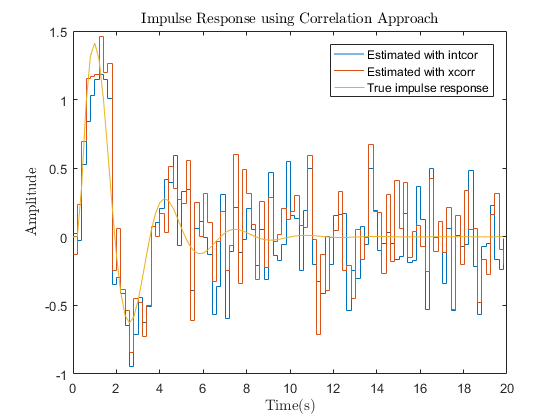
\includegraphics[height=9cm]{images/impulse_corr_app}
    \caption{Impulse response by the mean of the correlation approach calculated with intcor() and xcorr() against the real response.}
    \label{fig:corr_app}
\end{figure}

\begin{lstlisting}[language=Matlab,numbers=left,caption=Correlation approach,label=lst:corr_app]
% input signal
Uprbs = 0.5* prbs(7,4);
Te = 0.2; % sample time
N = length(Uprbs);
sim_time = N*Te;

% simulation
simin = struct();
simin.signals = struct('values', Uprbs);
simin.time = linspace(0,sim_time, N);
sim('ce1_1_sim')

% extract one period of the signals
N = length(Uprbs)/4;
Uprbs = Uprbs(1:N);
Y = simout(end+1-N:end)/Te;
time = simin.time(1:N);

% Correlation approach using intcor
Ruu = intcor(Uprbs, Uprbs);
Ryu = intcor(Y, Uprbs);
U = toeplitz(Ruu);
theta_intcor = pinv(U)*Ryu;

% Correlation approach using xcorr
Ryu = xcorr(Y, Uprbs);
Ruu = xcorr(Uprbs, Uprbs);
U = toeplitz(Ruu);
theta_xcorr = pinv(U)*Ryu;

G = tf([4],[1 1 4], 'InputDelay', Te);
Z = c2d(G, Te, 'zoh');
[G_impulse, G_time] = impulse(Z, time(end));

% error
err_intcor = norm(theta_intcor(1:127) - G_impulse)
err_xcorr = norm(theta_xcorr(1:127) - G_impulse)
\end{lstlisting}


\end{document}
